\section{Rewrite Rules}%
\label{rewrite-rules}

In this section, we will introduce the set of rules that transforms the ZX calculus from simply notation into a language \cite{Wetering2020}.

\notation{We will refer to the rules by some shorthand notation above equal signs. Note that this could refer to applying the rule in either direction.}

\subsection{Spider Fusion}%
The most fundamental rule of the ZX calculus is the \textit{spider fusion rule} (\textit{f}). It states that spiders of the same colour connected by one or more wires fuse and their phases add modulo $2\pi$ \cite{Wetering2020}.

\begin{figure}[H]
    \centering
    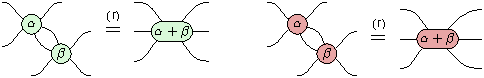
\includegraphics[width=0.75\textwidth]{chapter-2/fusion}
    \caption{Spider fusion rule for $Z$ spiders (left) and $X$ spiders (right).}
    \label{spider-fusion}
\end{figure}

It is the generalisation of adding the phases of successive rotations of the Bloch sphere. We can use this rule to identify commutation relations such as $Z$ rotations commuting through CNOT controls, and $X$ rotations, through CNOT targets.

% \vspace{5pt}
\includezxdiagram{chapter-2/cnot_commutation}{0.8}

%%%

\subsection{Identity Removal}%

The \textit{identity rule} (\textit{id}) states that any two-legged spider with no phase ($\alpha = 0$) is equivalent to a rotation by 0 radians, or identity.

\begin{figure}[H]
    \centering
    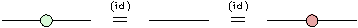
\includegraphics[width=0.6\textwidth]{chapter-2/identity}
    \caption{Identity removal rule.}
    \label{identity}
\end{figure}

Combining this with the spider fusion rule (\ref{spider-fusion}), we see that two successive rotations with opposite phases is equivalent to an empty wire.

\includezxdiagram{chapter-2/cancelling_rotations}{0.7}

%%%

\subsection{State Copy and $\pi$ Copy Rules}%

We can depict the $Z$ and $X$ eigenstates by assigning a phase to a $Z$ or an $X$ spider, respectively, through a Boolean variable $a$ (0 or 1) multiplied by $\pi$ \cite{Wetering2020}.

\includezxdiagramtext{chapter-2/boolean_x}{0.075}{
\ket 0 \text{ where $a = 0$ and }
\ket 1 \text{ where $a = 1$}}
%
\includezxdiagramtext{chapter-2/boolean_z}{0.075}{
\ket + \text{ where $a = 0$ and }
\ket - \text{ where $a = 1$}}

The $\pi$ \textit{copy rule} (\textit{c}) states that when a Pauli $Z$ or Pauli $X$ gate is pushed through a spider of the opposite colour, it is copied on all other legs and negates the spider's phase. A similar \textit{state copy rule} (\textit{c}) applies to the $Z$ and $X$ eigenstates.

\begin{figure}[H]
    \centering
    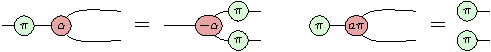
\includegraphics[width=0.9\textwidth]{chapter-2/pi_state_copy}
    \caption{$\pi$ copy (left) and state copy (right) rules for Pauli $Z$ gate and $Z$ eigenstates.}
    \label{state-copy}
    \label{pi-copy}
\end{figure}

%%%

\subsection{Hadamard Rules}

The Hadamard gate is both unitary and Hermitian. Therefore, we define the \textit{Hadamard self-inverse rule} (\textit{hi}).

\begin{figure}[H]
    \centering
    \includezxdiagram{chapter-2/hadamard_inverse}{0.42}
    \caption{Hadamard self-inverse rule.}
    \label{hadamard-self-inverse}
\end{figure}

Recalling that the Hadamard generator changes the colour of a spider and is self-inverse, we define the \textit{Hadamard commutation rule} (\textit{hi}).

\begin{figure}[H]
    \centering
    \includezxdiagram{chapter-2/hadamard_copy}{0.7}
    \caption{Hadamard commutation rule.}
    \label{hadamard-commutation}
\end{figure}

%%%

\subsection{Bialgebra Rule}

Using the spider fusion rule (\ref{spider-fusion}), we can show that a spider with two inputs and one output behaves like a classical XOR gate when applied to the eigenstates of the \textit{same} basis. Whilst using the state copy rule (\ref{state-copy}), we can show that a spider with one input and two outputs behaves like a classical COPY gate when applied to the eigenstates of the \textit{opposite} basis.

\begin{figure}[H]
    \centering
    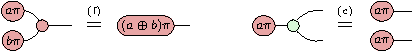
\includegraphics[width=0.7\textwidth]{chapter-2/xor_copy}
    \caption{XOR gate (left) and COPY gate (right) with respect to the $Z$ eigenstates.}
    \label{xor}
    \label{copy}
\end{figure}

Hence, using the natural commutation relation of the classical XOR and COPY gates, we define the \textit{bialgebra rule} (\textit{ba}). We encourage the reader to verify this relation.

\begin{figure}[H]
    \centering
    \includezxdiagram{chapter-2/bialgebra}{1}
    \caption{The bialgebra rule (and its classical motivation).}
    \label{bialgebra}
\end{figure}

%%%

\subsection{Hopf Rule}

Like with the bialgebra rule, our motivation for this rule stems from the behaviour of the classical XOR and COPY gates. Since copying two bits then taking their XOR invariably yields 0, we can define the \textit{Hopf rule} (\textit{hpf}).

\begin{figure}[H]
    \centering
    \includezxdiagram{chapter-2/hopf}{1}
    \caption{The Hopf rule (and its classical motivation).}
    \label{hopf}
\end{figure}

%%%

\newpage
\section{Conjugating with Paulis and Cliffords}

In this section we will develop several results later used in this thesis.
- Pauli Y gate
- conjugation by XPlus and XMinus
- conjugation by hadamards
- refer to zxfermion

Next, using the $\pi$ copy rule (\ref{pi-copy}), we can show that conjugating a $Z$ rotation by Pauli $X$ gates, negates the phase of the rotation, $\alpha \rightarrow -\alpha$.

\includezxdiagram{chapter-4/phase_flip}{0.7}
